\section{Protocolo IP}

La \textbf{capa de enlace} (capa 2) se encarga de proveer conectividad entre nodos adyacentes o vecinos, siendo responsable de transmitir una trama sobre un enlace en particular. Los mensajes entre origen y destino pueden transitar por distintas capas de enlace. La \textbf{Capa de Red} se encuentra por encima de la capa de enlace.

\begin{figure}[htbp]
    \centering
    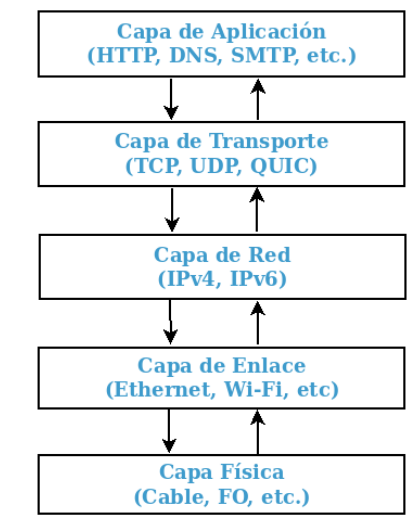
\includegraphics[width=0.5\textwidth]{capitulos/capitulo-1/imagenes/capas.png}
    \caption{Modelo TCP/IP}
    \label{fig:capas-de-modelo-tcp}
\end{figure}

\subsection{Diseño y Servicios}

La capa de red fué diseñada para que cumpla con los siguientes requerimientos: 

\noindent
\begin{enumerate}[label=\textcolor{acento}{$\bullet$}]
    \item Independiente de la tecnología de subred.
    \item Aislada de la cantidad, tipo y topologías de las \textbf{subredes}.
    \item Direccionamiento uniforme.
\end{enumerate}

Como servicios, debe poder transportar mensajes desde un nodo emisor a receptor (inclusive si son redes distintas) y determinar el camino que seguirá un mensaje entre dos nodos. Al no ser orientado a conexión, no brinda ni control de errores, ni secuenciamiento ni confiabilidad: es un servicio de \textbf{Best-Effort}.

\begin{definicion}{Protocolo Best-Effort}
    Hay independencia en cuanto al envío a través de la red, haciendo posible que los paquetes puedan llegar desordenados o seguir caminos diferentes. Tampoco hay control de errores. 
\end{definicion}

\newpage

Tiene dos funcionalidades principales:

\begin{itemize}[label=\textcolor{acento}{$\bullet$}]
    \item Direccionamiento
    \item Ruteo
\end{itemize}

También se encarga de multiplexar o demultiplexar protocolos superiores, y puede fragmentar paquetes.

\begin{figure}[htbp]
    \centering
    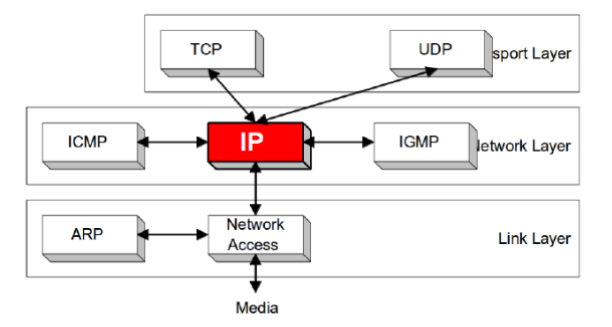
\includegraphics[width=0.5\textwidth]{capitulos/capitulo-1/imagenes/capas-relativo-ip.png}
    \caption{Modelo TCP/IP}
    \label{fig:capas-relativo-ip}
\end{figure}

\subsection{Estructura del Datagrama IP}

El \textbf{Datagrama IP} tiene longitud variable. Está compuesto por dos partes: header y payload. El \textbf{Header} tiene una longitud de entre 20 y 60 bytes.

\begin{figure}[htbp]
    \centering
    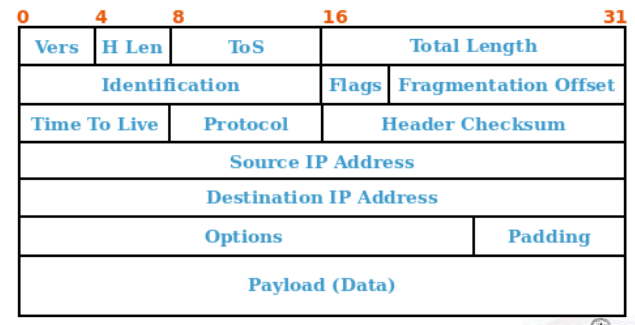
\includegraphics[width=0.5\textwidth]{capitulos/capitulo-1/imagenes/ip-datagram.png}
    \caption{Datagrama IP}
    \label{fig:ip-datagram}
\end{figure}

Los campos más relevantes son: 

\begin{itemize}[label=\textcolor{acento}{$\bullet$}]
    \item \textbf{Header Lenght:} longitud del header, en palabras de 32 bits.
    \item \textbf{Type of Service (TOS):} confiabilidad, prioridad, retardo y throughput.
    \item \textbf{Identification:} número único para segmentos del mismo datagrama.
    \item \textbf{Flags:} 
    \begin{itemize}[label=\textcolor{primario!60}{$\bullet$}]
        \item X = reservado. 
        \item D = Don't Fragment. Si es 0 puede fragmentarse, si es 1 no.
        \item M = More Fragments. Si es 0 es el último fragmento, si es 1 no.
    \end{itemize}
    \item \textbf{Fragment Offfset:} el desplazamiento del segmento dentro del datagrama original. Está dado en múltiplos de 8 bytes.
    \item \textbf{Time To Live (TTL):} número que se decrementa cada vez que llega a un router, y cuando llega a 0 se descarta. Es utilizado para evitar loops.
    \item \textbf{Protocol:} protocolo contenido en el campo de datos (UDP, TCP, ICMP, ...).
\end{itemize}

\subsection{Direccionamiento IP}

Las direcciones IP identifican unívocamente una intefraz de red. Los routers pueden tener más de una dirección IP. 









